\begin{figure*}
\centering
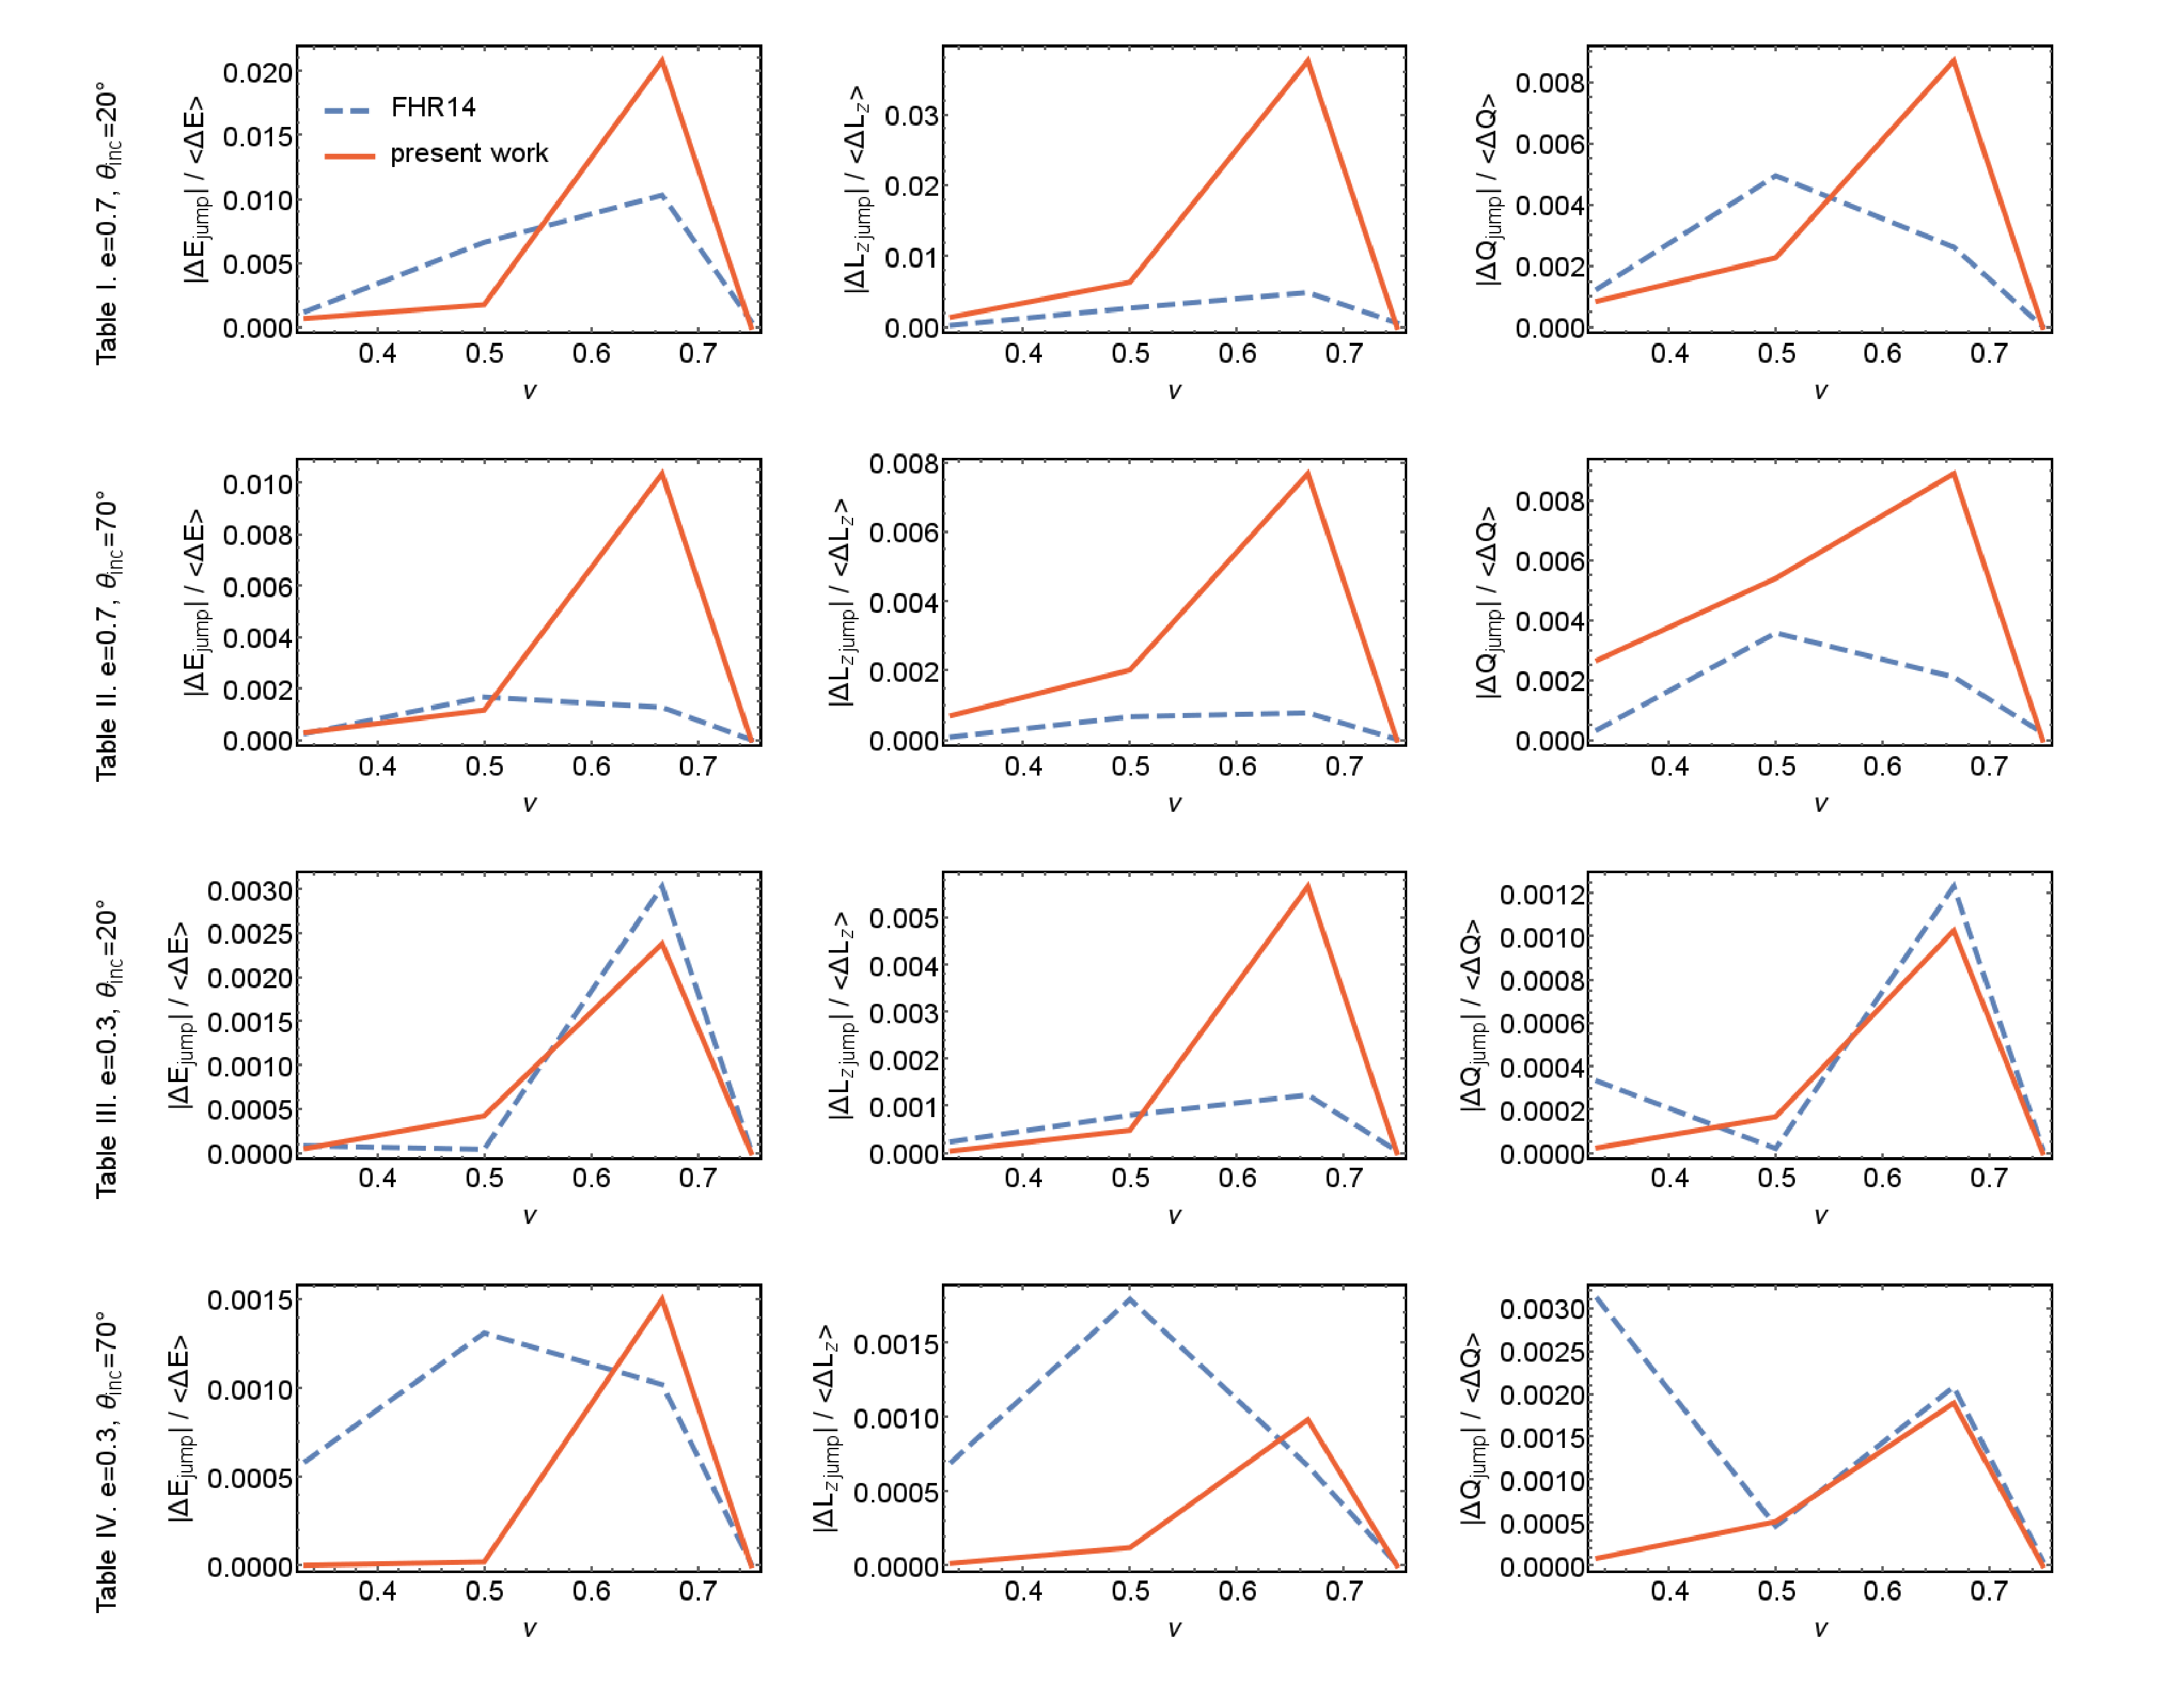
\includegraphics[width=\textwidth]{res_flux_FHR}
\caption{\label{fig:res-flux-FHR}Relative flux enhancements of $E$ (left column), $L_z$ (middle) and $Q$ (right) for resonance ratios corresponding to the 1:3, 1:2, 2:3 and 3:4 resonances. We show results as computed here with a solid red line, and results from Flanagan, Hughes and Ruangeri (FHR14)~\cite{Flanagan2012a} with a dashed blue line. Each row has a different eccentricity and inclination corresponding to tables I--IV in FHR14. All systems have $a_\ast=0.9$.}
\end{figure*}

The plus-polarisation of the GW at the start and end of the evolution is shown in the top row of \figref{good-waveform}.
\begin{figure*}
\centering
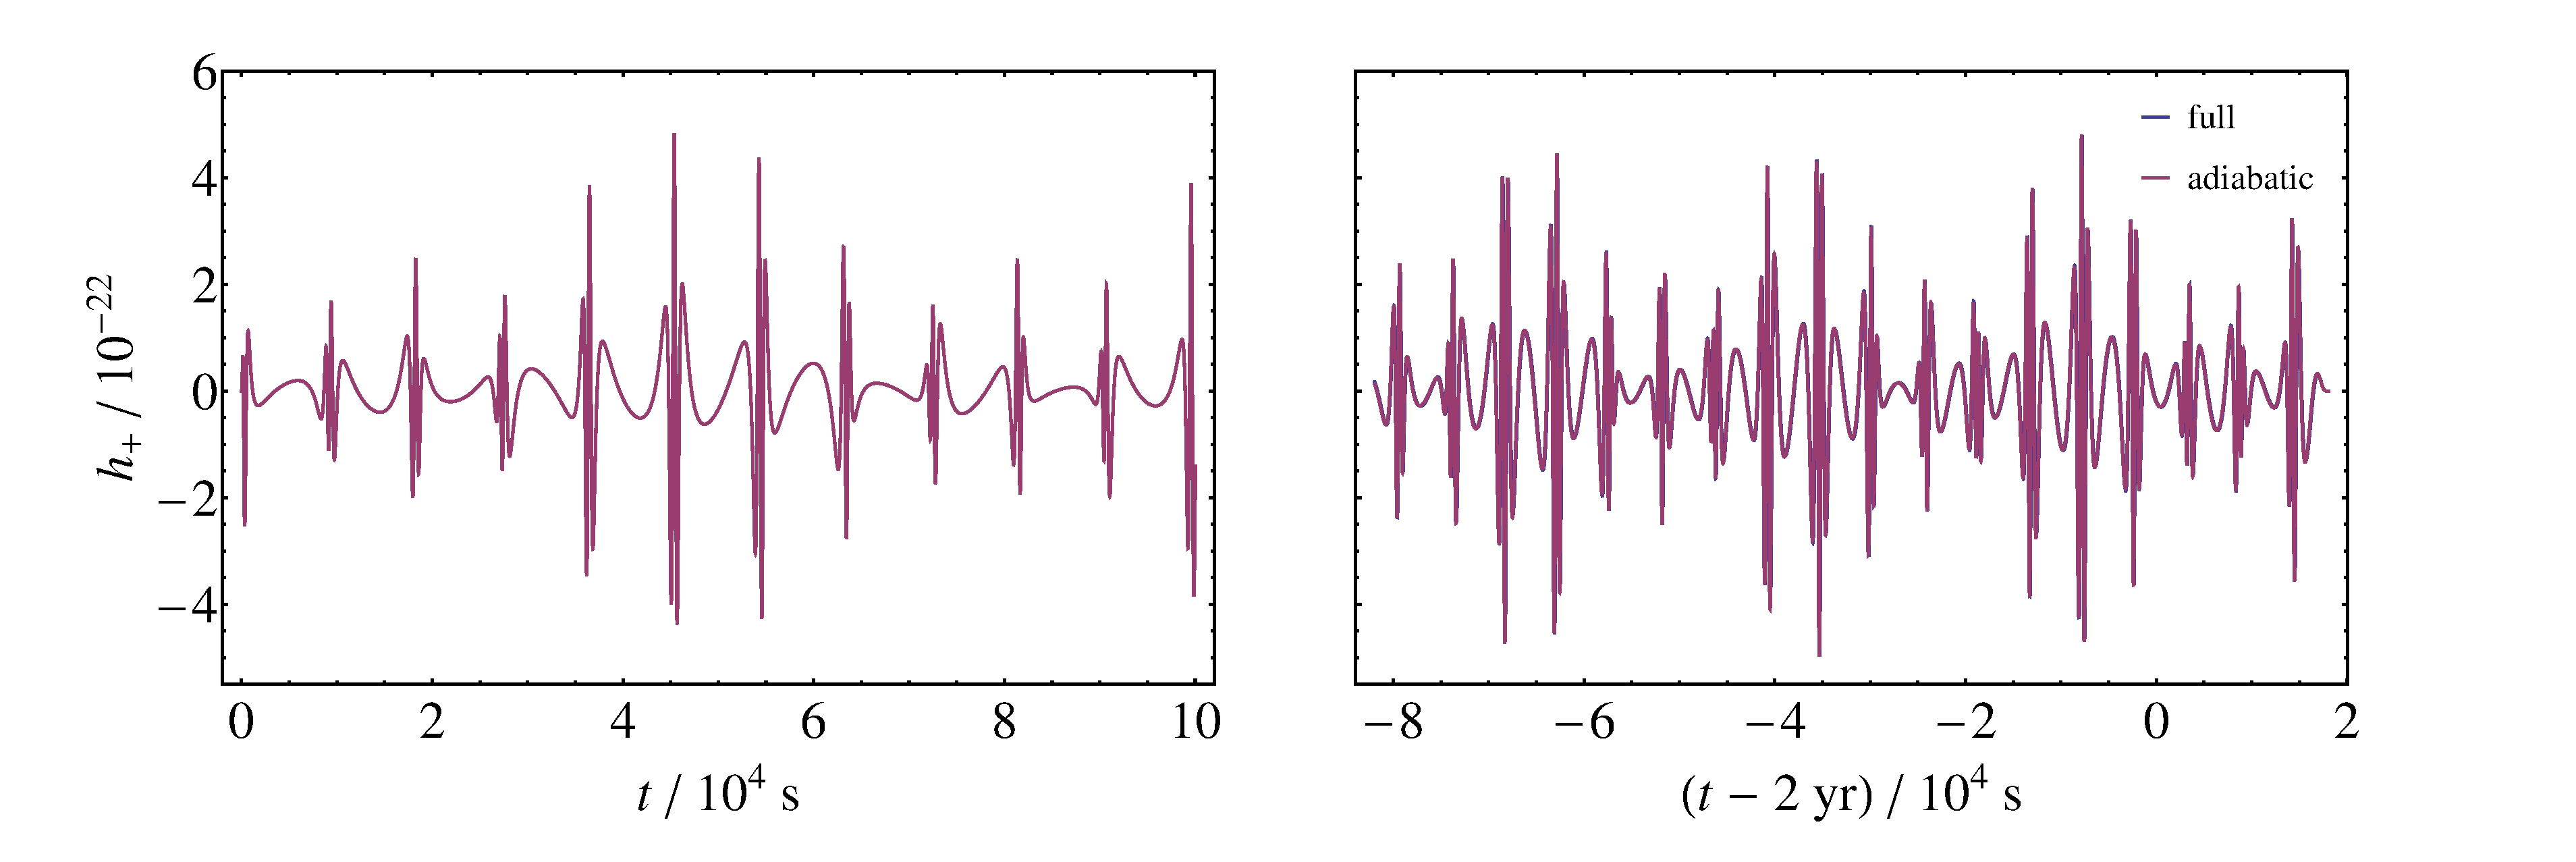
\includegraphics[width=0.92\textwidth]{Fig_good_waveform}
\caption{\label{fig:good-waveform}The plus-polarised waveform for an illustrative EMRI system with initial semi-latus rectum $p_0=7.5$, shown for two short segments at the start and end of a $2$ year evolution. The full and adiabatic models are both shown, but are indistinguishable by eye.}
\end{figure*}

Plotting the plus-polarised GWs at the start and end of the evolution, as before, demonstrates this dephasing, as shown in \figref{dephased-waveform}.
\begin{figure*}
\centering
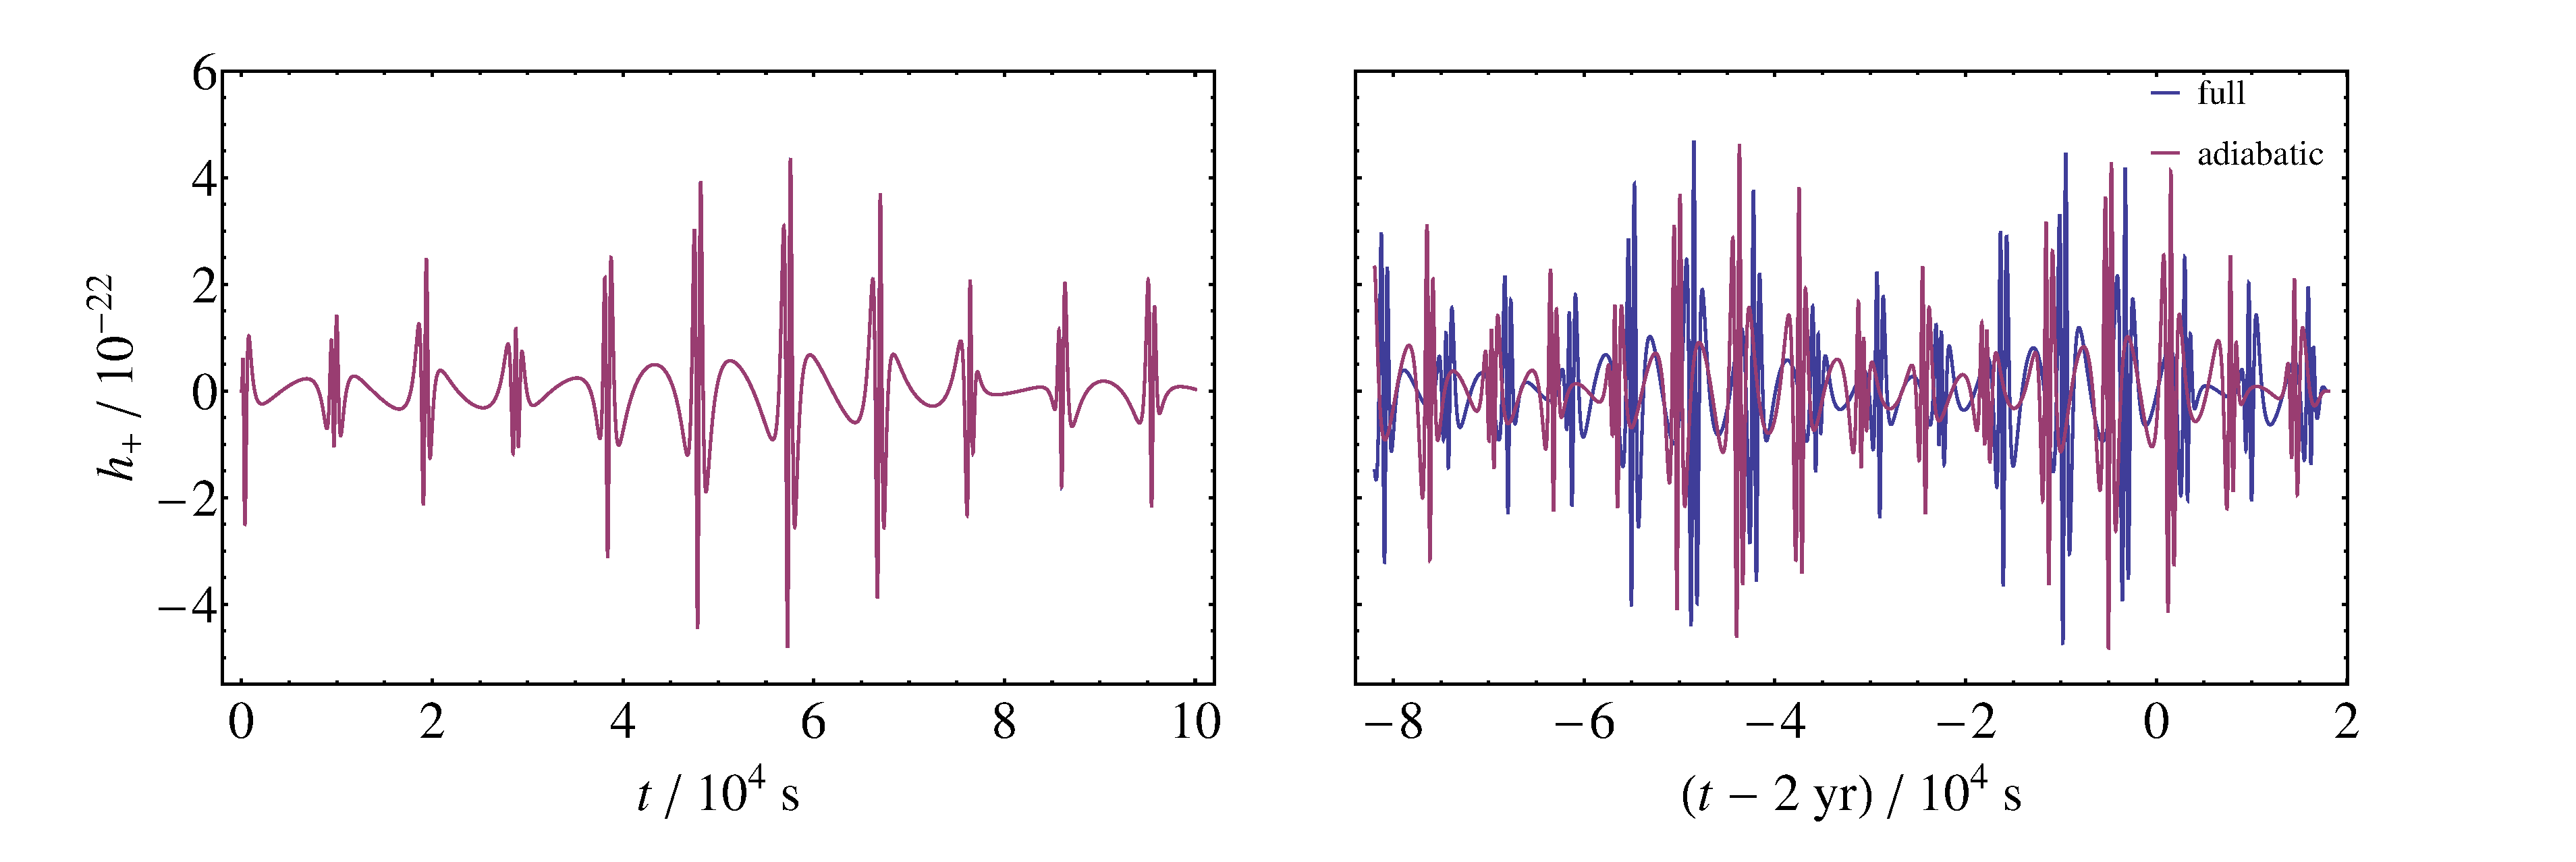
\includegraphics[width=0.92\textwidth]{Fig_dephased_waveform}
\caption{\label{fig:dephased-waveform}The plus-polarised waveform for an illustrative EMRI system with $p=7.85$, shown for two short segments at the start and end of a $2$ year evolution. The full and adiabatic models are both shown; there is a significant dephasing between them by the end of the evolution.}
\end{figure*}
